% Created by Jim Finnis
% Date Wed Feb 24 13:48:57 2021


\section{The data model}
The data model consists of two parts --- the data itself (largely
image cube data) and the graph. By far the most important kind of data
from the point of view of this document is the image data, which ties
into the user interface in complex ways. Other forms of data do exist,
but these are much simpler.

\subsection{ImageCube}
Most classes making up the image data 
model are described in the \texttt{pancamimage.py} file, including the main \texttt{ImageCube}
class. Some additional classes describing where images can come from are in \texttt{channelsource.py}.
The model is shown in outline in Fig.~\ref{image.png} although some links to channel sources
and mapping from nodes are omitted; these will be explained later.

\begin{figure}[ht]
\center
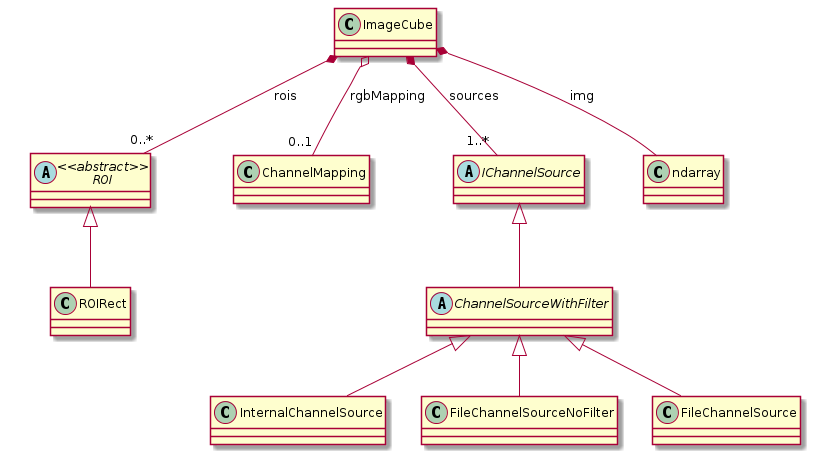
\includegraphics[width=5in]{image.png}
\caption{Outline UML class diagram of image model}
\label{image.png}
\end{figure}

The main class is \texttt{ImageCube}: this encapsulates a numpy array
\texttt{img}
which is the actual image data cube in the form
of a $w \times h \times depth$ array. The data type is 32-bit floating
point, and images are typically normalized to the range [0,1].

\begin{notebox}
In this document I have a tendency to refer to image data as both ``image'' and ``image cube.''
Both terms refer to the same thing: an array of floating point image data, with 1 or more channels
of information. There is no upper limit on the number of channels in an image (or image cube)
beyond system memory.
\end{notebox}


\subsection{IChannelSource and implementations}
Each \texttt{ImageCube} has a number of channels, and for each channel there must be a corresponding
entry in the \texttt{sources} list. This describes where that channel came from, so that (typically) filter
information can be preserved, where appropriate, through the graph. The sources for each channel are a set
of \texttt{IChannelSource} objects. For example, if an image was loaded through the RGB loader, it might
have three ``fake'' channel sources for red, green and blue. Thus the sources will be 
\begin{v}
[ {RED}, {GREEN}, {BLUE} ]
\end{v}
i.e.\ a list of three sets, each with a single source.
If the image is then converted to greyscale, this could
become
\begin{v}
[ {RED,GREEN,BLUE}, {RED,GREEN,BLUE}, {RED,GREEN,BLUE} ]
\end{v}
because each channel now contains information from the red, green and blue channels in the source file.
The \texttt{RED}, \texttt{GREEN} and \texttt{BLUE} values refer in this case to \texttt{FileChannelSourceNoFilter} objects
which contain ``fake'' filter information and a filename identifier.
Each \texttt{IChannelSource} contains methods for accessing:
\begin{itemize}
\item an \textbf{identifier string} for the source from which the channel was acquired (typically a filename or data ID);
\item a \textbf{filter} and methods for obtaining the filter name, filter position and an actual filter reference (for extra data such as centre wavelength) (note
that much of this information will be ``fake'' for images loaded from plain RGB files);
\item methods for getting string descriptors for this source.
\end{itemize}

Nodes generate and process this information in different ways. For example, a \emph{gradient} node takes a single channel and converts it into an RGB image with
a colour gradient: here, the output image's sources are ``internal RGB'' sources with no identifier or sensible filter data because the output's colour
is entirely artificial. In contrast, a the \emph{curve} for performing a sigmoid function on all channels of an image will give the output image the
same sources as the input image.

Sources are used to keep track of each channel as it moves through the graph so they can be processed and displayed appropriately:
Fig.~\ref{app.png} shows a typical node in the ``node controls and output'' section. This section, as it does in many nodes,
contains a ``canvas'' displaying an image. Above the canvas are three combo boxes which select the channels in the image cube to display on the canvas,
and these are typically labelled by a string generated from the source data for each channel (along with the index). Sources are also used
to select channels to combine and manipulate in those nodes which do so.

\subsection{RGB channel mappings}
The previous section briefly mentions the three RGB mapping combo boxes at the
top of the canvas component in the node controls in Fig~\ref{app.png}. In
canvases --- components which display images --- a multi-channel image cube
must be displayed as RGB data. The combo boxes control how this is done, and
the data is made persistent in a slightly complicated way, as shown in Fig.~\ref{rgb.png}.

\begin{figure}[ht]
\center
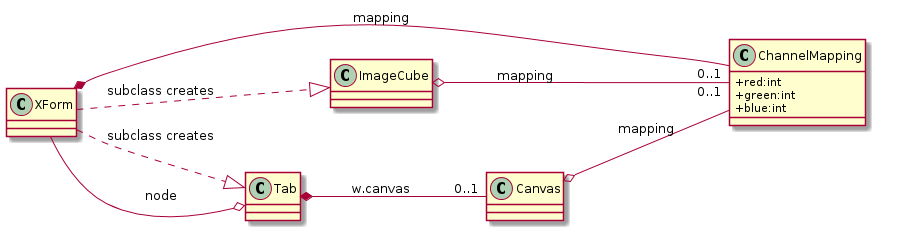
\includegraphics[width=5in]{rgb.png}
\caption{RGB mapping classes}
\label{rgb.png}
\end{figure}

The relationships will hopefully become clearer when I come to describe how nodes work in more
detail, but for now:
\begin{itemize}
\item A \texttt{ChannelMapping} object consists of three integers giving the indices of 
the channels in an image cube to display in the red, green and blue channels on screen.
\item An \texttt{XForm} (i.e.\ a node) may need to show an image on a canvas. If so, it 
will use the \texttt{mapping} field in \texttt{XForm} to store a mapping. This is provided
as a convenience, not all node classes will use it, and some may need to create more if they 
display more than one image.
\item When an \texttt{XForm} creates an image for display or passes
one through, it sets the mapping of the image to the mapping of the node. This is used in the
\texttt{rgb()} method to generate the RGB representation.
\item When an \texttt{XForm} is opened for modification, it creates a subclass of \texttt{Tab}.
This will contain a \texttt{Canvas}, which is given a reference to the mapping inside the
\texttt{XForm}. It needs this so that the mapping can be modified even when no image is present.
\end{itemize}
This may seem rather redundant, but
\begin{itemize}
\item We need the mapping to be owned by the node, so it can be serialised and persists when
there is no image and no open tab.
\item We need to have a reference to the mapping in the canvas, so it can be manipulated by
the combo boxes even when no image is present.
\item Finally, we need a reference to the mapping in the image so that \texttt{rgb()} can be called
on the image when it is input into another node. This is used in nodes like \emph{inset}, which
operate entirely on RGB representations --- it's much neater if these are the RGB representations
output by the nodes which feed in.
\end{itemize}




\subsection{Regions of interest}
Regions of interest belong to images, and modify how nodes process those images. They are added to 
images by region of interest nodes such as \emph{rect}. Figs.~\ref{app.png} and \ref{graph.png}
show this in action:
\begin{itemize}
\item A file is read in, producing an image cube
\item A \emph{rect} node adds a region of interest to this image. The outputs are:
\begin{itemize}
\item the image with the rectangle added to its list of ROIs;
\item the image cropped to the bounding box of the list of ROIs (at the moment, just this rectangle)'
\item an RGB representation of the image (according to the previous node's canvas RGB mapping);
annotated with the rectangle and some text, and also an ROI added describing the rectangle;
\item the rectangle datum itself.
\end{itemize}
\item a \emph{decorr stretch} takes the annotated RGB representation output and imposes a decorrelation
stretch --- but only on the regions of interest in the image (in this case, inside the rectangle)
\item a \emph{histequal} node performs a histogram equalisation, again honouring the regions of interest
which have been passed through the previous node unchanged.
\end{itemize}
As shown in Fig.~\ref{image.png}, each image contains a list of \texttt{ROI} objects,
each of which is an instantiation of a subclass of \texttt{ROI}. 

To honouring regions of interest inside a node's \texttt{perform()} method:
\begin{itemize}
\item \texttt{ImageCube.subimage()} will return a \texttt{SubImageCubeROI} object. This encapsulates
a numpy array containing the image bounded to a rectangle around the regions of interest and
a boolean mask (again as a numpy array) specifying which pixels in this rectangle are actually
in regions of interest.
\item The manipulation can now be performed on the \texttt{img} field of this ``subimage,'' but
only on those pixels whose values are true in the corresponding \texttt{mask} field.
\item The modified pixels can be ``spliced'' into the original image cube, creating a new image
cube, using the \texttt{modifyWithSub} method.
\end{itemize}
This example shows the operation of the decorrelation stretch:
\begin{lstlisting}[language=Python]
    def perform(self,node):
        img = node.getInput(0)
        if img is None:
            node.img = None
        elif not node.enabled:
            node.img = img
        elif img.channels != 3:
            ui.error("Can't decorr stretch images with other than 3 channels")
        else:
            subimage = img.subimage()
            newimg = decorrstretch(subimage.img, subimage.mask)
            node.img = img.modifyWithSub(subimage, newimg)
        if node.img is not None:
            node.img.setMapping(node.mapping)
        node.setOutput(0, node.img)
\end{lstlisting}
There are several checks for whether the node is actually enabled, and whether there is an image
present to stretch, but the core lines are these:
\begin{lstlisting}[language=Python]
            subimage = img.subimage()
            newimg = decorrstretch(subimage.img, subimage.mask)
            node.img = img.modifyWithSub(subimage, newimg)
\end{lstlisting}
The \texttt{decorrstretch} takes two arguments: the numpy array containing the pixels which bound
the ROIs, and the mask for those pixels in that array which are in the ROIs. It returns an image
of the same size, which is then spliced back into the original image. The new image returned
will have the same channel sources, the same ROIs and the same RGB mapping.

\begin{notebox}
Much of the ROI system is work in progress, particularly combining
multiple ROIs. This documentation might change.
\end{notebox}
